% Created by Chris Chronopoulos (chrono@leaflabs.com) on 20140930
% 

% ***********************************************************
% ******************* PHYSICS HEADER ************************
% ***********************************************************
% from http://www.dfcd.net/articles/latex/latex.html
% ***********************************************************
% Version 2
\documentclass[11pt]{article} 
\usepackage{amsmath} % AMS Math Package
\usepackage{amsthm} % Theorem Formatting
\usepackage{amssymb}	% Math symbols such as \mathbb
\usepackage{graphicx} % Allows for eps images
\usepackage{multicol} % Allows for multiple columns
\usepackage[dvips,letterpaper,margin=0.75in,bottom=0.75in]{geometry}
\usepackage{amsmath}
\usepackage{graphics}
\usepackage{graphicx}
\usepackage{epsfig}
\usepackage{verbatim}
\usepackage{listings}
\usepackage{enumerate}
\usepackage[authoryear]{natbib} % can't get this to work?
\usepackage{hyperref} % i think there's a conflicting command here?
 % Sets margins and page size
% \pagestyle{empty} % Removes page numbers
\makeatletter % Need for anything that contains an @ command 
\renewcommand{\maketitle} % Redefine maketitle to conserve space
{ \begingroup \vskip 10pt \begin{center} \large {\bf \@title}
	\vskip 10pt \large \@author \@date \end{center}
  \vskip 10pt \endgroup \setcounter{footnote}{0} }
\makeatother % End of region containing @ commands
%\renewcommand{\labelenumi}{(\alph{enumi})} % Use letters for enumerate
% \DeclareMathOperator{\Sample}{Sample}
\let\vaccent=\v % rename builtin command \v{} to \vaccent{}
\renewcommand{\v}[1]{\ensuremath{\mathbf{#1}}} % for vectors
\newcommand{\gv}[1]{\ensuremath{\mbox{\boldmath$ #1 $}}} 
% for vectors of Greek letters
\newcommand{\uv}[1]{\ensuremath{\mathbf{\hat{#1}}}} % for unit vector
\newcommand{\abs}[1]{\left| #1 \right|} % for absolute value
\newcommand{\avg}[1]{\left< #1 \right>} % for average
\let\underdot=\d % rename builtin command \d{} to \underdot{}
\renewcommand{\d}[2]{\frac{d #1}{d #2}} % for derivatives
\newcommand{\dd}[2]{\frac{d^2 #1}{d #2^2}} % for double derivatives
\newcommand{\pd}[2]{\frac{\partial #1}{\partial #2}} 
% for partial derivatives
\newcommand{\pdd}[2]{\frac{\partial^2 #1}{\partial #2^2}} 
% for double partial derivatives
\newcommand{\pdc}[3]{\left( \frac{\partial #1}{\partial #2}
 \right)_{#3}} % for thermodynamic partial derivatives
\newcommand{\ket}[1]{\left| #1 \right>} % for Dirac bras
\newcommand{\bra}[1]{\left< #1 \right|} % for Dirac kets
\newcommand{\braket}[2]{\left< #1 \vphantom{#2} \right|
 \left. #2 \vphantom{#1} \right>} % for Dirac brackets
\newcommand{\matrixel}[3]{\left< #1 \vphantom{#2#3} \right|
 #2 \left| #3 \vphantom{#1#2} \right>} % for Dirac matrix elements
\newcommand{\grad}[1]{\gv{\nabla} #1} % for gradient
\let\divsymb=\div % rename builtin command \div to \divsymb
\renewcommand{\div}[1]{\gv{\nabla} \cdot #1} % for divergence
\newcommand{\curl}[1]{\gv{\nabla} \times #1} % for curl
\let\baraccent=\= % rename builtin command \= to \baraccent
\renewcommand{\=}[1]{\stackrel{#1}{=}} % for putting numbers above =
\newtheorem{prop}{Proposition}
\newtheorem{thm}{Theorem}[section]
\newtheorem{lem}[thm]{Lemma}
\theoremstyle{definition}
\newtheorem{dfn}{Definition}
\theoremstyle{remark}
\newtheorem*{rmk}{Remark}
% added by CKC
\newcommand{\amom}{\mathcal{L}}
\newcommand{\flux}{\mathcal{F}}
\newcommand{\laplacian}[1]{\nabla^2 #1}


% ***********************************************************
% ********************** ENDcit HEADER *************************
% ***********************************************************

\usepackage{bm}

\title{Willow GUI User Guide}
\date{\today}

\begin{document}
\maketitle

%%%%%%%%%%%%%%%%%%%%%%%%%%%%%%%%%%%%%%%%%%%%%%%%%%%%%%%%%%%%%%%%%%%%%%%%%%%%%%%%%

\section{Introduction}
\label{sec_intro}

This is the user guide for the Willow GUI --- a desktop application for interacting with Willow, a 1024-channel electrophysiology system developed by LeafLabs (www.leaflabs.com) in collaboration with MIT's Synthetic Neurobiology Group (SNG). This document, which is contained in the source code repository in \texttt{docs/user\_guide/}, contains information for end-users. Developers should check out the developer's guide, which can be found in \texttt{docs/dev\_guide/}.

%%%%%%%%%%%%%%%%%%%%%%%%%%%%%%%%%%%%%%%%%%%%%%%%%

\section{System Overview}
\label{sec_overview}

Willow is based on a Spartan 6 FPGA which collects and routes data from up to 32 amplifier/digitizer chips (Intan RHD2132), each chip sampling 32 channels of electrophysiology signals. The primary purpose of the hardware is to record all 1024 channels of data directly to an SSD, which is connected via SATA interface to the Willow board. A photograph of the bare hardware, connected and ready to record from a single headstage, is shown in Figure~\ref{fig_hw}.

\begin{figure}[h!]
\begin{center}
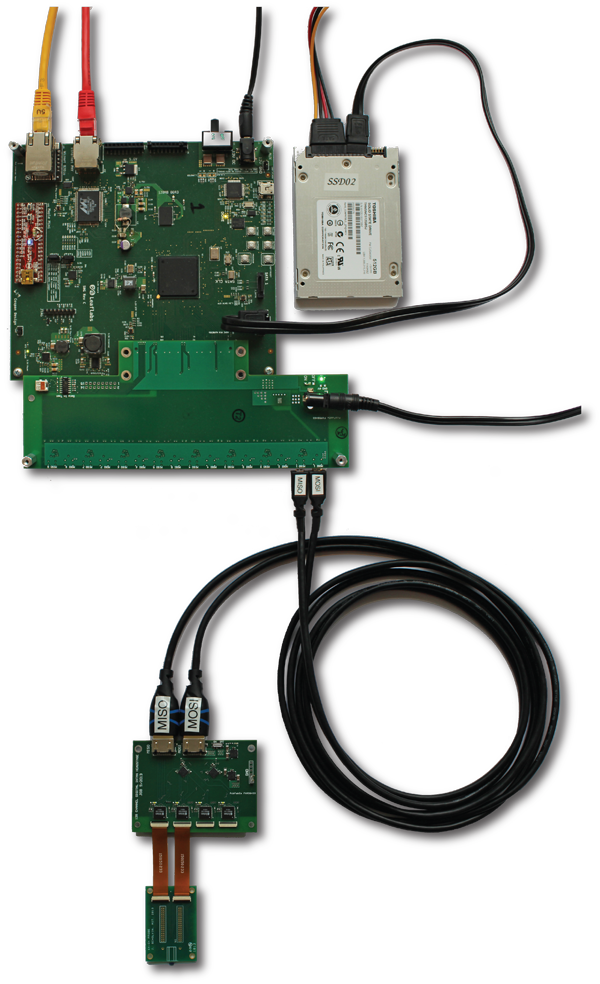
\includegraphics[width=6cm]{screenshots/full_setup.png}
\end{center}
\caption{Willow hardware with a single headstage connected.}
\label{fig_hw}
\end{figure}

The Willow board communicates over TCP and UDP connections with a workstation computer running a daemon server called \texttt{leafysd}. All interactions with the hardware go through the daemon, which exposes an interface based on Google's Protocol Buffers (protobuf). The daemon repository includes command-line utilities for sending and receiving protobuf messages to and from the daemon. The GUI was designed to replace the command-line workflow with a more accessible and streamlined graphical approach.

There are many layers to the full Willow system; to learn more about them in detail, see \texttt{wired-leaf-docs/user\_guide}. For the end-user, however, it is sufficient to be familiar with the basic architecture of the system. Namely, that the only robust mode of data acquisition is recording, which saves data directly to the SSD, and not to the workstation. To tighten the feedback look for data validation, there are other modes of acquisition (namely streaming and snapshots) which route data directly to the workstation, but these are not robust to data loss. For scientific experiments, the workflow is: record to SATA disk, then transfer over to a workstation for analysis. This is further explained in Section~\ref{sec_usage}.

%%%%%%%%%%%%%%%%%%%%%%%%%%%%%%%%%%%%%%%%%%%%%%%%%%%%%%%%%%%%%%%%%%%%%%%%%%%%%%%%%

\section{Setup}
\label{sec_setup}

This setup guide assumes you have already installed the daemon and configured your network; if not, refer to the Willow user guide in \texttt{wired-leaf-docs/user\_guide}.

\subsection{Obtaining the GUI}
\label{sec_setup_obtaining}

To access the GUI repository, you'll need to be given permissions on the server --- to request access, email \texttt{neuro@leaflabs.com}. Once you have permissions, you can clone the repo like so

\vspace{5mm}
\texttt{\$ git clone git@git.leaflabs.com:sng-gui}
\vspace{5mm}

\subsection{Dependencies}
\label{sec_setup_deps}

Before running the GUI, install these mandatory dependencies:

\vspace{5mm}
\texttt{\$ sudo apt-get install python-numpy python-matplotlib python-qt4 python-h5py \textbackslash}

\hspace*{20mm}\texttt{python-progressbar}
\vspace{5mm}

\subsection{Configuration}
\label{sec_setup_config}

The GUI uses a configuration file, \texttt{src/parameters.py}, which stores variables related to the daemon installation, data storage, and other parameters. Before running the GUI, open \texttt{src/parameters.py} in an editor and modify the \texttt{DAEMON\_DIR} and \texttt{DATA\_DIR} variables to point to the locations of the \texttt{sng-daemon} repo and the preferred top-level data directory on your system.

%%%%%%%%%%%%%%%%%%%%%%%%%%%%%%%%%%%%%%%%%%%%%%%%%

\section{Usage}
\label{sec_usage}

To run the GUI:

\vspace{5mm}
\texttt{\$ cd src/}

\texttt{\$ ./main.py}
\vspace{5mm}

\noindent
The GUI will present its main window (Figure~\ref{fig_mainwindow}), which consists of a tab dialog and a message log. The daemon is automatically started in the background, with \texttt{stderr} and \texttt{stdout} redirected to \texttt{log/eFile} and \texttt{log/oFile}, respectively. The message log should display a line indicating that the daemon was started successfully.

\begin{figure}[h!]
\begin{center}
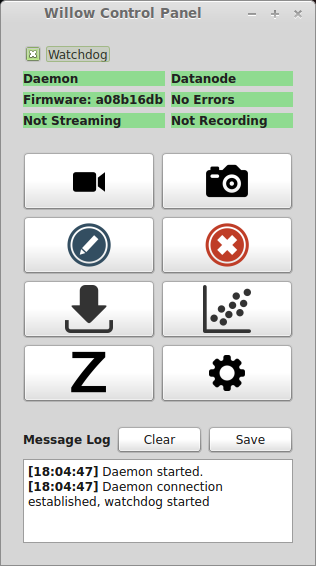
\includegraphics[width=8cm]{screenshots/mainwindow.png}
\end{center}
\caption{GUI main window, immediately after startup.}
\label{fig_mainwindow}
\end{figure}

\subsection{Acquire Tab}
\label{sec_usage_acquire}

The first tab that is presented when the GUI starts up is the Acquire Tab. It encapsulates the tasks that deal with the data acquisition (DAQ) module on the Willow hardware. Anything that involves interaction with the Intan chips will be found in the Acquire Tab.

There are three modes of operating the DAQ: streaming, snapshot, and recording. These can be done simultaneously, with exception that you cannot take a snapshot while streaming; if you try, the GUI will refuse, printing a message to let you know.

\subsubsection{Streaming}
\label{sec_usage_acquire_streaming}

Streaming is the real-time visualization of data from the Intan chips. When streaming, the data acquired from the ADC's is routed directly to the GUI, without being saved to SATA. Currently, users can view one channel at a time, as a scrolling waveform in a stream window.

To launch a stream window, click ``Launch Stream Window'' in the Acquire Tab. You will be presented with a dialog (Figure~\ref{fig_streamdialog}) to configure the stream parameters. Fill in the channel number you want to view, the plotting range, and the refresh rate --- or, accept the default values and click ``OK''. The stream window will appear (Figure~\ref{fig_streamwindow}), though it will not be streaming yet. To start/stop the stream, use the ``Start'' and ``Stop'' buttons. You can also navigate the plot, even while streaming, using the Navigation Toolbar at the bottom of the stream window. To undo/redo navigation changes, use the back and forward arrows; to return to the original view, click the home icon.

\begin{figure}[h!]
\begin{center}
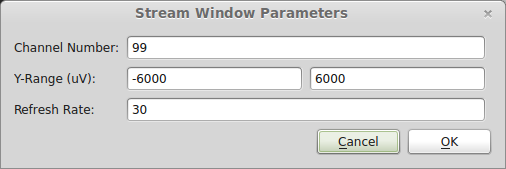
\includegraphics[width=12cm]{screenshots/streamdialog.png}
\end{center}
\caption{Stream window configuration dialog.}
\label{fig_streamdialog}
\end{figure}

Live streaming in matplotlib is reasonably CPU intensive, so you may want to pause the stream while running other tasks within the application. Adjusting the ``refresh rate'' parameter in the stream dialog may help alleviate performance issues.

\begin{figure}[h!]
\begin{center}
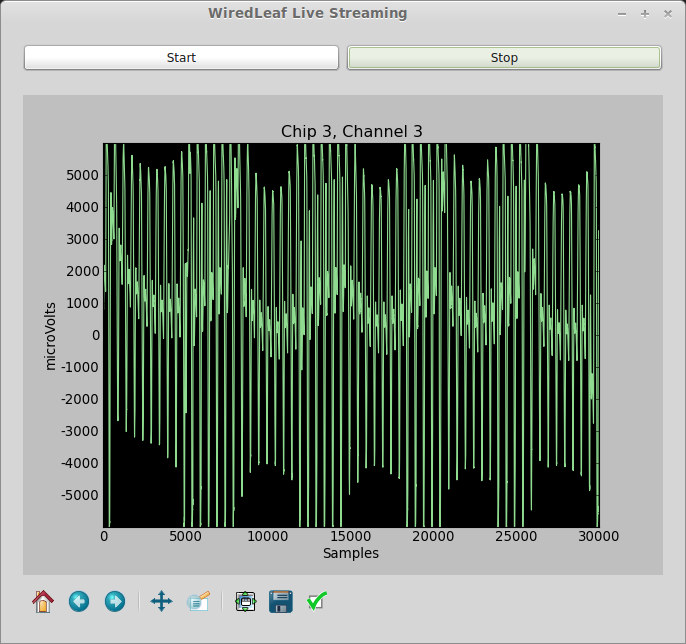
\includegraphics[width=12cm]{screenshots/streamwindow.png}
\end{center}
\caption{Stream window showing 60 Hz noise from a bare Intan chip.}
\label{fig_streamwindow}
\end{figure}

\subsubsection{Snapshots}
\label{sec_usage_acquire_snapshot}

A snapshot is a short (\textless~10 second) acquisition of board samples (all 1024 channels) which is saved directly to the workstation. It is essentially a stream which gets saved to a file (HDF5 format by default) to be analyzed offline. Like streaming, taking a snapshot does not involve the SATA drive, so you can take snapshots without worrying about overwriting your experiment on disk.

To take a snapshot, first make sure that any Stream Windows are stopped; then click ``Take Snapshot'' in the Acquire Tab. You will be presented with a dialog (Figure~\ref{fig_snapshotdialog}) to configure the snapshot. Fill in the number of samples you want to acquire (remember that 1 second = 30000 samples), and the filename you want to save to, and click ``OK''. The default filename is generated from your \texttt{DATA\_DIR} variable and a timestamp taken at the moment you clicked ``Take Snapshot'' --- the format is \texttt{DATA\_DIR/snapshot\_YYYYMMDD-hhmmss.h5}, so the filename should be unique up to 1 second of granularity.

The snapshot dialog also gives you the option to ``Plot when finished'' by checking the box in the lower-left corner. If this is selected, then after the snapshot is saved, the GUI will automatically import the file and present it in a Plot Window (refer to Section~\ref{sec_usage_plot} for information on using the Plot Window).

\begin{figure}[h!]
\begin{center}
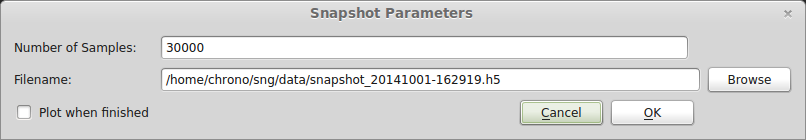
\includegraphics[width=14cm]{screenshots/snapshotdialog.png}
\end{center}
\caption{Snapshot dialog.}
\label{fig_snapshotdialog}
\end{figure}

\subsubsection{Recording}
\label{sec_usage_acquire_recording}

Recording is the acquisition of data directly to the SATA disk. It is the only acquisition mode that is guaranteed to be robust, and is intended for scientific experiments. To start a recording, click ``Start'' on the Acquire Tab. The large status box will turn from gray to red, and the disk usage bar will start advancing to indicate how much disk space is left (Figure~\ref{fig_recording}). To stop recording, click ``Stop''.

\vspace{5mm}
\noindent \textbf{IMPORTANT:} Every time you click ``Start'', the system will start recording from the beginning of the disk, over-writing any previous experiments you may have recorded. If you've just recorded an experiment and want to preserve the data, it is recommended that you \underline{transfer} the data over to your workstation immediately after clicking ``Stop'' (see Section~\ref{sec_usage_transfer}). If storage space is an issue on your workstation, an alternative is to remove the SATA disk and label it, thus repurposing the disk buffer as an archival system.

\begin{figure}[h!]
\begin{center}
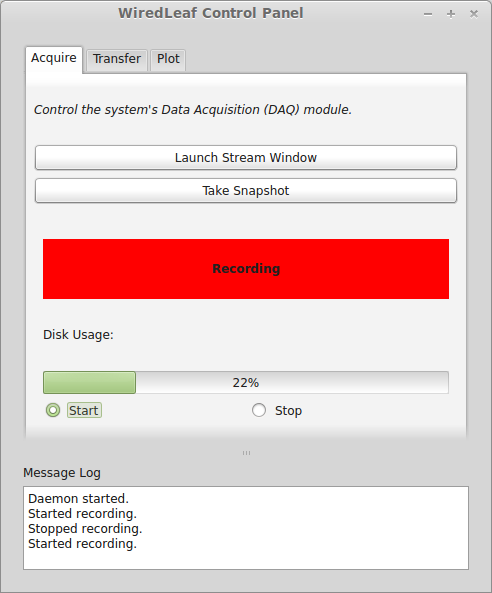
\includegraphics[width=8cm]{screenshots/recording.png}
\end{center}
\caption{A recording in progress.}
\label{fig_recording}
\end{figure}

\subsection{Transfer Tab}
\label{sec_usage_transfer}

The Transfer Tab is used to transfer an experiment from the SATA disk to the workstation's file system. An experiment must be transferred over before it can be analyzed --- but even if analysis is not immediately necessary, it is wise to transfer important experiments over as soon as they are recorded, because (as explained in Section~\ref{sec_usage_acquire_recording}) experiments on disk are in danger of being over-written by subsequent recordings.

To perform a transfer, enter the number of samples you want to transfer over (remember that 1 second = 30000 samples), or leave the field blank to transfer the entire experiment on disk. Then, choose a target filename, and click ``Transfer Data''. The GUI (and the hardware) will be unavailable until the transfer is complete.

Transfer times are approximately equal to recording times; if your recording lasted $n$ minutes, you can expect to wait $\sim n$ minutes for a transfer to complete. To get some estimate of how long is the experiment on disk, click ``Determine Lenght of Experiment on Disk'' near the top of the Transfer Tab. This will perform a binary search to determine where the experiment ends, and then print out the result, along with the ``experiment cookie'', which is the Unix timestamp from the moment the experiment was begun. The binary search takes about 30 seconds; an example of the resulting information is shown in Figure~\ref{fig_transfertab}.

\begin{figure}[h!]
\begin{center}
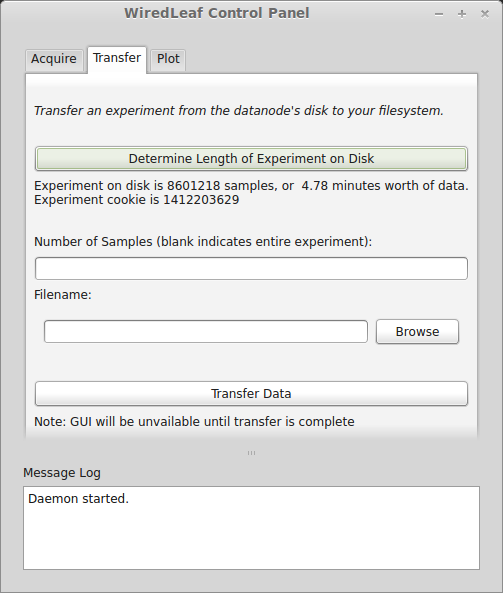
\includegraphics[width=8cm]{screenshots/transfertab.png}
\end{center}
\caption{The Transfer Tab, with binary search results showen.}
\label{fig_transfertab}
\end{figure}

\subsection{Plot Tab}
\label{sec_usage_plot}

The Plot Tab is used to import data files (either snapshots or recordings) into Plot Windows for inspection. To open a Plot Window, enter a filename (either manually or using the Browse button), select whether you want the entire data set or just a subset, and click ``Launch''. The software will load the data into memory (this can take a while for large data sets --- a progress bar indicates the status of the import operation) and present a Plot Window.

\subsubsection{Plot Window}
\label{sec_usage_plot_plotwindow}

The Plot Window (Figure~\ref{fig_plotwindow}) allows you to view the data in some detail as an array of 1-dimensional waveforms. A control panel at the top allows you to adjust how many channels are shown at once, which bank of channels is currently being displayed, and the range of the plotting axes. A ``bank'' here represents a contiguous, ordered set of $n$ channels, where $n$ can range from 1 to 16. To page through banks, use the spinbox in the control panel --- when activated, it can be controlled using the arrow keys on your keyboard.

\begin{figure}[h!]
\begin{center}
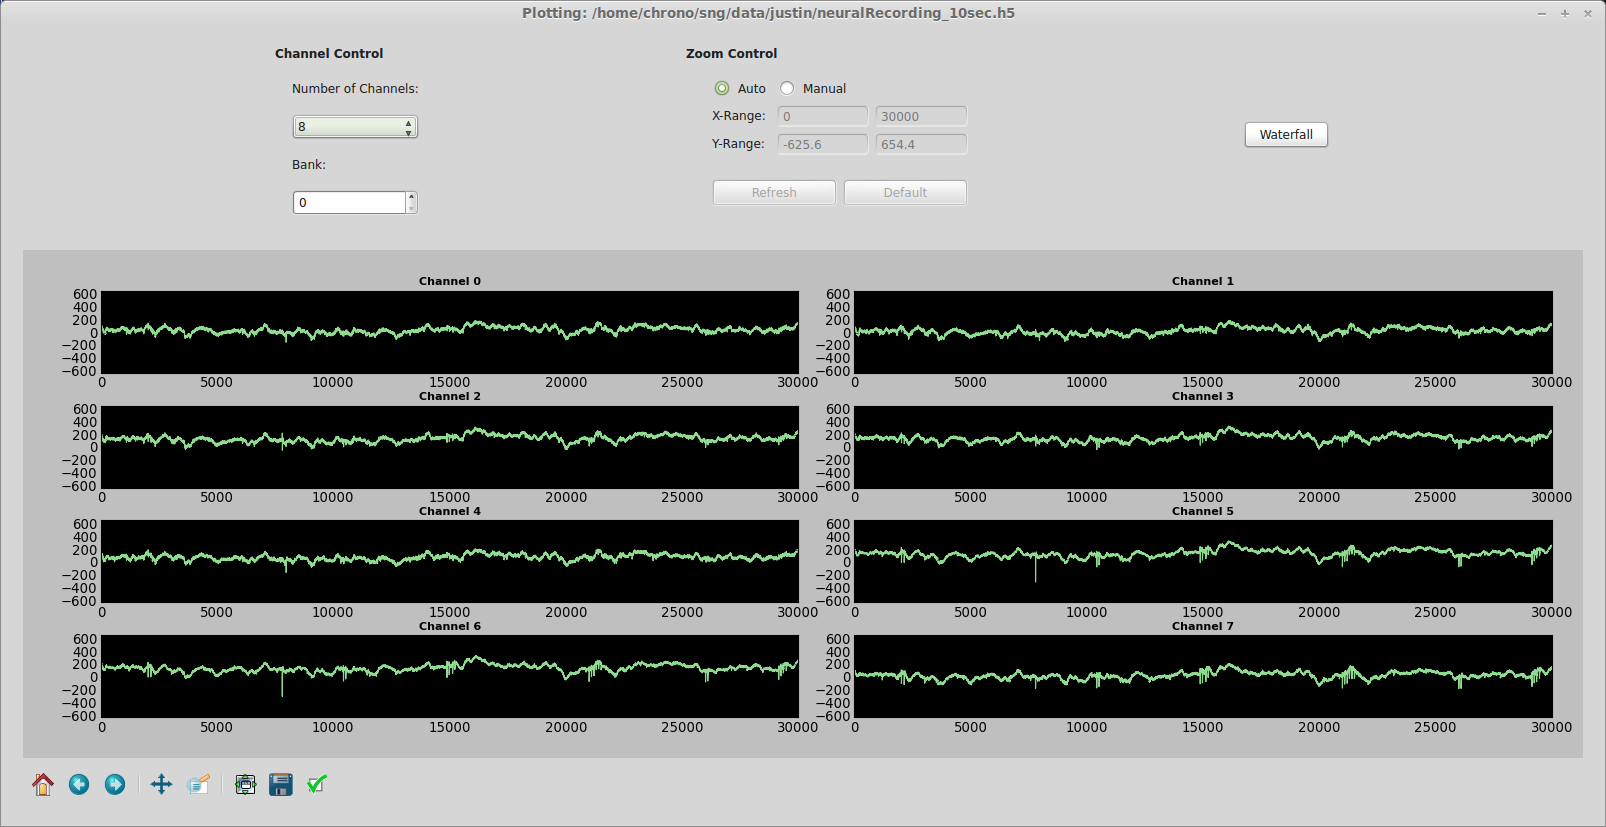
\includegraphics[width=17cm]{screenshots/plotwindow.png}
\end{center}
\caption{The Plot Window.}
\label{fig_plotwindow}
\end{figure}

The ``Zoom Control'' section allows you to set the plotting range of \textbf{all} plots in the window simultaneously. By default, the zoom mode is ``Auto'', which looks at the current bank of channels and chooses a $y$-range based on its min and max; the auto-range updates every time you advance banks, or change the number of channels displayed. In ``Manual'' mode, you can set exactly the $x$-range and $y$-range of all the plots in the array --- just enter the extrema and click ``Refresh''. Another way to adjust the plots is by using the Navigation Toolbar at the bottom of the window. This allows you to zoom in on one plot in particular, leaving the others unchanged. To get back to the zoom settings defined by the ``Zoom Control'' group, just click the home icon.

Near the top-right corner of the Plot Window, you'll find a button labeled ``Waterfall''. Click here to launch the Waterfall Plot Window.

\subsubsection{Waterfall Plot Window}
\label{sec_usage_plot_waterfall}

The Waterfall Plot Window (Figure~\ref{fig_waterfall}) shows \textbf{all} the data from a given import, in a 2-dimensional color plot. The $x$-axis is time (with units in sample number), the $y$-axis is channel number, and color represents signal (voltage), with values indicated by the colorbar on the right.

\begin{figure}[h!]
\begin{center}
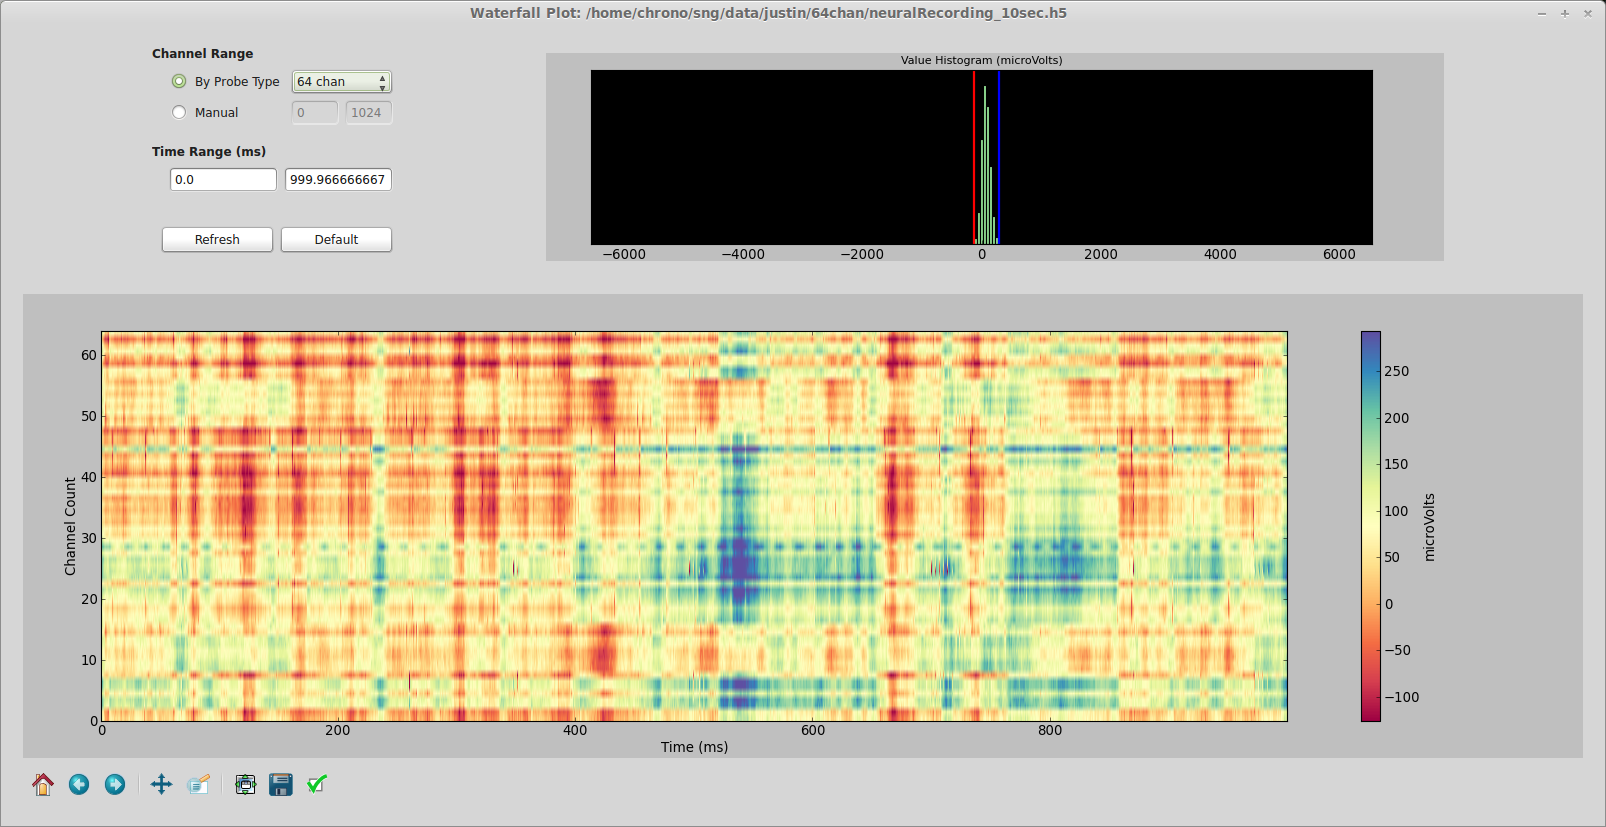
\includegraphics[width=17cm]{screenshots/waterfall.png}
\end{center}
\caption{Waterfall Plot Window.}
\label{fig_waterfall}
\end{figure}

When you first open the Waterfall Plot Window, it will show the entire 1024-channel dataset. If some (or most) of those channels were not connected to a live Intan chip, they will show up as zeros, which will appear as a large black band on the Waterfall Plot. To zoom in on the channels of interest, adjust the ``Y-Range'' parameters in the control panel at the top. As usual, you can also zoom into subregions of the plot by using the Navigation Toolbar at the bottom. And finally, it's likely that you will want to adjust the limits of the color mapping to bring out interesting features in your data set. In Figure~\ref{fig_waterfall_zoom}, we have used these techniques to zoom in on a spike train that registered across several channels.

\begin{figure}[h!]
\begin{center}
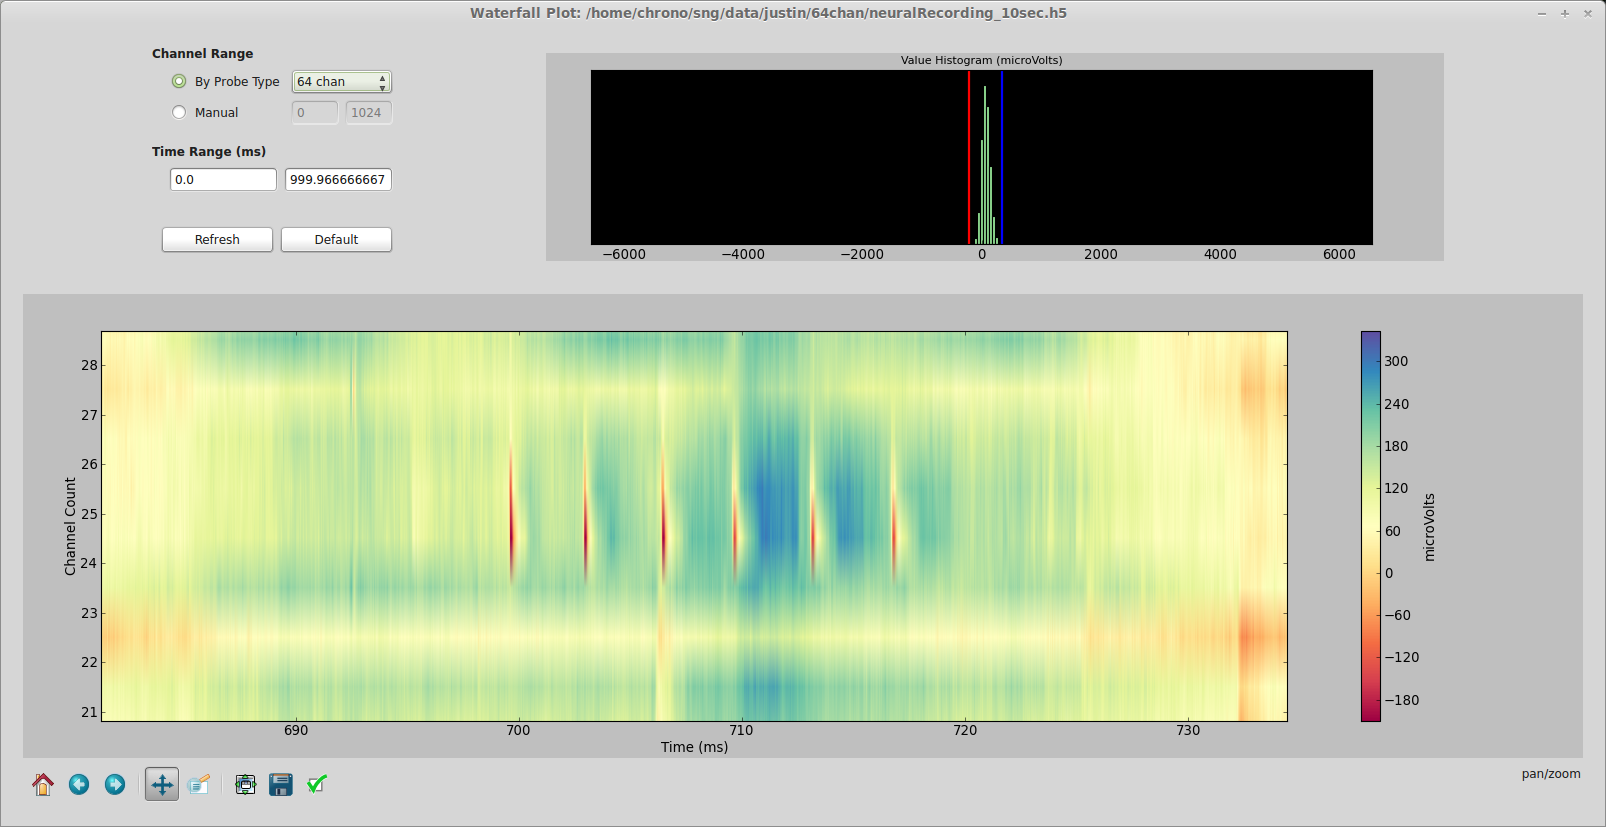
\includegraphics[width=17cm]{screenshots/waterfall_zoom.png}
\end{center}
\caption{A train of 6 spikes, shown on several channels in the Waterfall Plot.}
\label{fig_waterfall_zoom}
\end{figure}


%%%%%%%%%%%%%%%%%%%%%%%%%%%%%%%%%%%%%%%%%%%%%%%%%

\end{document}





